\section{Correcting vignetting effect on a PSP system}

Depending on the object, two methods for background subtraction may be performed for correcting vignetting effect. These techniques may be applied depending upon the range of height variation of a test object. 

\subsection{Direct Background Subtraction}

For plane/flat surfaces with minimal details of relative uniform depth, we used the resulting phase map itself to serve as the background. 
We took the mean of its small blocks (m x n pixels) and applied bicubic interpolation. The block size was carefully chosen so as not to remove the details.
The interpolated image is then subtracted to the unprocessed phase map. We refer to this process as the Direct Background Subtraction (DBS) method.

\subsection{Reference Background Subtraction}

A different approach was used for objects of nonuniform depth/height. 
DBS may only be used for this type if phase unwrapping is done per region, i.e. nonuniform illumination is less apparent if not observable for a subregion of an image; hence, it will be easier to correct it without deforming the details (modified DBS).

However, this is a tedious and highly time consuming process especially for large images and thus, we disregarded this method. As a resolution, a white image (unto which PSP is also performed) was used as the reference and its unwrapped phase was subsequently subtracted to that of the object's unwrapped phase and we call this the Reference Background Subtraction (RBS) method.

\subsection{3D reconstruction}
Figure \ref{fig:stone} shows the reference and object unwrapped phases of the pebbled wall portion. 
We see a nonuniform phase for the reference's unwrapped phase even if it is supposed to be a flat white image.

\captionsetup[figure]{width=5in}
\begin{figure}[h!]
	\centering
	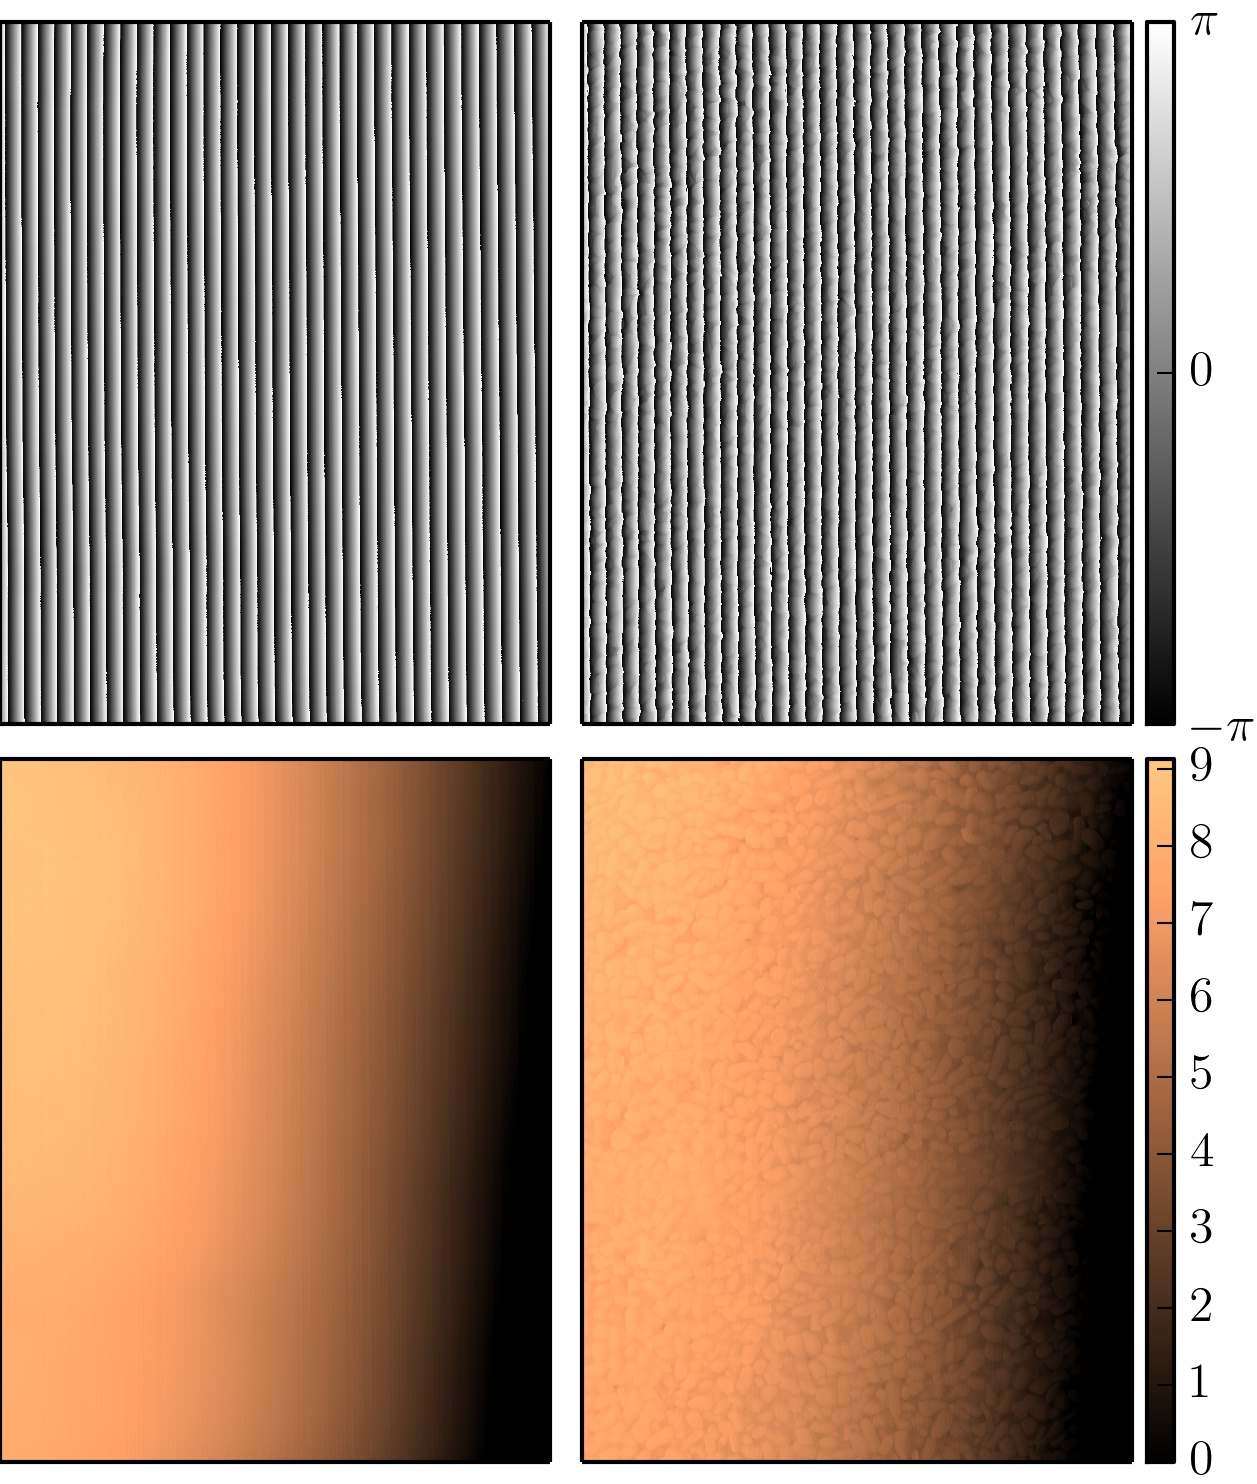
\includegraphics[width=0.62\textwidth]{figures/stone_copper.jpg}
	\caption{Wrapped (top) and unwrapped phase maps of the reference (right) and the pebbled wall (left). The images are displayed in `copper' colormap to match color of the actual object.}
	\label{fig:stone}
\end{figure}

This is an indication of the nonuniform illumination of light which is also seen in the object's unwrapped phase. 
Hence, the details of the pebbled wall are not observable.

RBS and DBS are implemented to the unwrapped phase of the pebbled wall. 
The details of the pebbled wall are now observable but the resulting phase map from using RBS still has an apparent nonuniform intensity while DBS is more uniform. 

\captionsetup[figure]{width=5in}
\begin{figure}[h!t]
	\centering
	\subfigure[]{\includegraphics[width=0.45\textwidth]{figures/stoneRBS.pdf}\label{fig:RBS}}
	\subfigure[]{\includegraphics[width=0.45\textwidth]{figures/stoneDBS.pdf}\label{fig:DBS}}
	\caption{Resulting phase maps after using (a) RBS and (b) DBS.}
	\label{fig:stoneBS}
\end{figure}

Shown in Figure \ref{fig:stonehist} is the histogram distribution of the phase values after application of RBS and DBS. We see that the RBS has a wider distribution of phase values as compared to DBS. The standard deivation of the two were also obtained: RBS = 0.315, DBS = 0.201. Higher standard deviation means a higher distribution of phase values (greater nonuniformity). 


\captionsetup[figure]{width=5in}
\begin{figure}[h!]
	\centering
	\includegraphics[width=0.75\textwidth]{figures/stonehisto.pdf}
	\caption{Histogram distribution of phase values of the pebbled wall after RBS and DBS from Figure~\ref{fig:DBS}.}
	\label{fig:stonehist}
\end{figure}

DBS is better for flat objects with minimal details (depth/height of less than 10 mm). As for RBS, incorrectly placing the reference during the experiment will lead to discrepancies in phase values.
